\begin{figure}[ht]
    \centering
    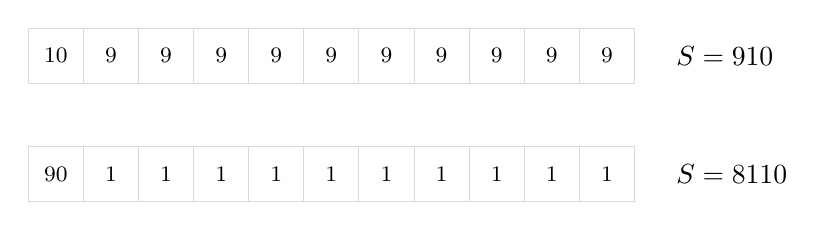
\begin{tikzpicture}[
        node distance=0pt,
        % Stile delle celle: bordo grigio chiaro e font sans-serif
        cell/.style={
            draw=black!15, 
            minimum size=0.7cm, 
            inner sep=0pt, 
            font=\footnotesize
        },
        header/.style={
            anchor=west
        },
        result/.style={
            anchor=west,
            xshift=0.4cm
        }
    ]
        
    \node[cell] (a0) at (0, 0) {10};
    \foreach \i [remember=\i as \last (initially 0)] in {1,...,10} {
        \node[cell] (a\i) at (\i*0.7, 0) {9};
    }
    \node[result] at (a10.east) {$S = 910$};


    \node[cell] (b0) at (0, -1.5) {90};
    \foreach \i [remember=\i as \last (initially 0)] in {1,...,10} {
        \node[cell] (b\i) at (\i*0.7, -1.5) {1};
    }
    \node[result] at (b10.east) {$S = 8110$};

    % --- SCENARIO B: Distribuzione Sbilanciata ---
    % \node[header, font=\small] at (0, -0.8) {Scenario B: Item counts (Skewed)};

    % Prima cella
    % \node[cell] (b1) at (0, -1.5) {90};
    
    % Ciclo per le altre 10 celle (valore 1)
    % \foreach \i [remember=\i as \last (initially 1)] in {2,...,11} {
    %     \node[cell, right=of b\last] (b\i) {1};
    % }

    % Risultato Surprise Number
    % \node[result] at (b11.east) {$S = 8,110$};

    \end{tikzpicture}
    
\end{figure}